% !TeX program = lualatex
% !TeX encoding = utf8
% !TeX spellcheck = uk_UA

\documentclass[]{article}
\usepackage[fontsize = 12pt]{fontsize}
\usepackage{ifluatex}

\ifluatex
	\usepackage{fontspec}
	\setsansfont{CMU Sans Serif}
	\setmainfont{CMU Serif}
	\setmonofont{CMU Typewriter Text}
	\defaultfontfeatures{Ligatures={TeX}}
	\usepackage[math-style=TeX]{unicode-math}
\else
	\usepackage[utf8]{inputenc}
	\usepackage[T2A,T1]{fontenc}
	\usepackage{cmap}
\fi
\usepackage[english, russian, ukrainian]{babel}

\usepackage{adjustbox}


\usepackage[%
	a4paper,%
	footskip=1cm,%
	headsep=0.3cm,%
	top=2cm, %
	bottom=2cm, %
	left=2cm, %
	right=2cm, %
    ]{geometry}
\renewcommand{\baselinestretch}{1}

\clubpenalty =10000
\widowpenalty=10000

\setlength{\parskip}{0.5ex}%
\setlength{\parindent}{2.5em}%

\usepackage{titlesec}


\titleformat{\section}{\normalfont\bfseries}{\thesection.}{1ex}{}
\titleformat{\subsection}{\small\bfseries}{\thesubsection.}{1ex}{}

\usepackage{tikz, pgfplots}

\usepackage[colorlinks=true,
	urlcolor = blue, %Colour for external hyperlinks
    linkcolor  = malina, %Colour of internal links
	citecolor  = green, %Colour of citations
	bookmarks = true,
	bookmarksnumbered=true,
	unicode,
	linktoc = all,
	hypertexnames=false,
	pdftoolbar=false,
	pdfpagelayout=TwoPageRight,
	pdfauthor={Ponomarenko S.M. aka sergiokapone},
	pdfdisplaydoctitle=true,
	pdfencoding=auto
	]%
	{hyperref}
		\makeatletter
	\AtBeginDocument{
	\hypersetup{
		pdfinfo={
		Title={\@title},
		}
	}
	}
	\makeatother
\usepackage{amsmath}

\usepackage[breakable, most, minted]{tcolorbox}
\usepackage{minted}

\newcounter{pythoncode}
\newtcblisting{pythoncode}{
    listing engine=minted,
    listing only,
    sharp corners,
    breakable,
    size=fbox,
    boxrule=1pt,
    pad at break*=1mm,
    colback=gray!5,
    colframe=gray,
    enhanced,
    minted language=python,
    minted options={
        autogobble,
        fontsize=\small,
        breaklines,
        style=emacs
    },
    overlay={
        \node[anchor=north east, font=\ttfamily\scriptsize, color=gray] at (frame.north west) {In [\thepythoncode]:\relax};
    },
    code={\stepcounter{pythoncode}}
}


\newtcblisting{out}{
    listing engine=minted,
    listing only,
    sharp corners,
    breakable,
    size=fbox,
    boxrule=1pt,
    pad at break*=1mm,
    colback=white,
    colframe=white,
    enhanced,
    minted language=python,
    minted options={
        autogobble,
        fontsize=\small,
        breaklines
    },
    overlay={
        \node[anchor=north east, font=\ttfamily\scriptsize, color=gray] at (frame.north west) {Out[\thepythoncode]:\relax};
    },
}



\title{Data Science. Домашнє №3}
\begin{document}

\maketitle

\section*{Імпорт модулів}

\begin{pythoncode}
import numpy as np
import pandas as pd
import matplotlib.pyplot as plt
from sklearn.linear_model import LinearRegression
\end{pythoncode}

\section*{Матриці}

Якщо у вас є набір даних з \(m\) вибірок, кожна з яких називається
\(x^{(i)}\) (\(n\)-вимірний вектор), і вектор результатів \$ Y \$
(\(m\)-вимірний вектор), можна побудувати наступні матриці:

\begin{enumerate}
	     \item  Матриця ознак


\begin{equation*}
\mathbf{X} =
	\begin{pmatrix}
		\vec{x}^{(1)} \\
		\vec{x}^{(2)} \\
		\vdots        \\
		\vec{x}^{(m)} \\
	\end{pmatrix}
	=
	\begin{pmatrix}
		1      & x_1^{(1)} & x_2^{(1)} & \ldots & x_n^{(1)} \\
		1      & x_1^{(2)} & x_2^{(2)} & \ldots & x_n^{(2)} \\
		\vdots & \vdots    & \vdots    & \ddots & \vdots    \\
		1      & x_1^{(m)} & x_2^{(m)} & \ldots & x_n^{(m)} \\
	\end{pmatrix}
\end{equation*}


	\item Вектор результатів


\[
	\vec{Y} =
	\begin{pmatrix}
		\vec{y}_1 \\
		\vec{y}_2 \\
		\vdots    \\
		\vec{y}_m \\
	\end{pmatrix}
\]

	\item Вектор вагових коефіцієнтів


\[
	\vec{w} =
	\begin{pmatrix}
		\vec{w}_0 \\
		\vec{w}_1 \\
		\vdots    \\
		\vec{w}_n \\
	\end{pmatrix}
\]

\end{enumerate}

\section*{Задача}

Наша задача --- проаналізувати, як залежить ціна на будинок \(h\)
залежно від площі \(x_1\), кількості ванних кімнат \(x_2\) та кількості
спалень \(x_2\).

\section{<<Self-made>> реалізація алгоритму градієнтного спуску}

\subsection{Функція гіпотези лінійної регресії}
Функція має вигляд: \[ \vec{h}(\vec{w}, X) = X \vec{w}, \] де $ \vec{w}
$ --- вектор вагових коефіцієнтів, \$ X \$ --- вектор-стовпець векторів
ознак (матриця ознак).

\begin{pythoncode}
def h(W, X):
    """
    Calculate the hypothesis for linear regression.

    Parameters:
    W (numpy.ndarray): Weight vector (dimension: (n+1,)).
    X (numpy.ndarray): Feature matrix (dimension: (m, n+1)).

    Returns:
    hypothesis (numpy.ndarray): Hypothesis values (dimension: (m,)).
    """
    return X @ W
\end{pythoncode}

\subsection{Функція втрат}

Функція має вигляд:

\[ J(\vec{w}) = \frac1{2m} \left( \vec{h}(\vec{w}, \mathbf{X}) - \vec{Y} \right)^2. \]

Функція втрати (loss function) є однією з ключових компонентів в задачах
машинного навчання і глибокого навчання, і вона виконує декілька
важливих функцій:

\begin{enumerate}
	\def\labelenumi{\arabic{enumi}.}
	\item
	      \textbf{Вимірювання помилки моделі}: Функція втрати визначає,
	      наскільки добре модель попереджує або класифікує дані в порівнянні зі
	      справжніми (очікуваними) значеннями. Вона обчислює різницю між
	      прогнозованими і справжніми результатами. Ця різниця, яку часто
	      називають ``помилкою'' або ``втратою'', вказує на те, наскільки
	      великою є розрозненість між моделлю та даними.
	\item
	      \textbf{Оптимізація моделі}: Однією з центральних задач в машинному
	      навчанні є оптимізація параметрів моделі так, щоб функція втрати була
	      мінімізована. Іншими словами, ми намагаємося знайти такі значення
	      параметрів моделі, які роблять прогнози якомога ближчими до справжніх
	      даних. Це досягається шляхом зменшення значення функції втрати.
	\item
	      \textbf{Оцінка якості моделі}: Функція втрати дозволяє оцінювати
	      якість моделі. Чим менше значення функції втрати, тим краще модель
	      вирішує задачу. Виміряння втрати на навчальних та тестових даних
	      допомагає визначити, наскільки добре модель узагальнює свої знання на
	      нових даних.
\end{enumerate}

\begin{pythoncode}
def J(W, X, Y):
    """
    Calculate the mean squared error (MSE) for linear regression.

    Parameters:
    W (numpy.ndarray): Weight vector (dimension: (n+1,)).
    X (numpy.ndarray): Feature matrix (dimension: (m, n+1)).
    Y (numpy.ndarray): Target vector (dimension: (m,)).

    Returns:
    mse (float): Mean squared error.
    """
    m = len(Y)  # Кількість навчальних прикладів
    error = h(W, X) - Y
    return 1 / ( 2 * m ) * error @ error
\end{pythoncode}

\subsection{Градієнт функції втрат}

Вектор-градієнт функції втрат має вигляд:

\[ \vec{\nabla} J = \frac1{m} \mathbf{X}^{\mathrm{T}} \cdot (\mathrm{X}\vec{w} - \vec{Y} )  = \frac1{m} \mathbf{X}^{\mathrm{T}} \cdot (\vec{h} - \vec{Y} ). \]

\textbf{Градієнт функції втрат} (gradient of the loss function) --- це
вектор, який показує напрямок та швидкість найшвидшого зростання функції
втрат в околицях поточного значення параметрів моделі. Іншими словаим,
це вектор, який показує, як зміниться значення функції втрат при дуже
невеликих змінах параметрів моделі.

Основні аспекти градієнту функції втрат:

\begin{itemize}
	\item
	      \textbf{Напрямок}: Градієнт вказує напрямок найшвидшого зростання
	      функції втрат. Якщо ви рухаєтесь в напрямку градієнту, то значення
	      функції втрат буде зростати найшвидше.
	\item
	      \textbf{Величина}: Модуль градієнту (його довжина) показує, наскільки
	      швидко зростає функція втрат в цьому напрямку. Більший градієнт вказує
	      на більш значущі зміни в функції втрат при малих змінах параметрів
	      моделі.
\end{itemize}

Використання градієнту функції втрат дуже важливо в процесі оптимізації
моделі, так як він вказує на те, які кроки (зміни параметрів) потрібно
зробити для покращення моделі. У методах оптимізації, таких як
стохастичний градієнтний спуск, градієнт використовується для оновлення
параметрів моделі з метою зменшення функції втрат.

\begin{pythoncode}
def nabla_J(W, X, Y):
    """
    Computes the gradient of the loss function for linear regression.

    Parameters:
    W (numpy.ndarray): Vector of weights (dimensionality (n+1,)).
    X (numpy.ndarray): Feature matrix (dimensionality (m, n+1)).
    Y (numpy.ndarray): Target value vector (dimensionality (m,)).

    Returns:
    Gradient (numpy.ndarray): The gradient of the loss function (dimension (n+1,)).
    """

    m = len(Y)  # Кількість навчальних прикладів
    error  = X.T @ (h(W, X) - Y)
    gradient = (1 / m) * error
    return gradient
\end{pythoncode}

\subsection{Функція градієнтного спуску}

Формула для обчислення вагових коефіцієнтів в результаті одного кроку
градієнтного спуску (одна ітерація) має вигляд:

\[ \vec{w} = \vec{w}_{\text{prev}} - \alpha \vec{\nabla} J \]

\begin{pythoncode}
def gradient_descent(X, Y,
                     alpha=0.001,
                     num_iterations=1_000,
                     epsilon=1e-7):
    """
    Perform gradient descent optimization for linear regression.

    Parameters:
    X (numpy.ndarray): Feature matrix (dimension: (m, n+1)).
    Y (numpy.ndarray): Target vector (dimension: (m,)).
    alpha (float, optional): Learning rate. Defaults to 0.001.
    num_iterations (int, optional): Number of iterations. Defaults to 1000.
    epsilon (float, optional): Convergence threshold. Defaults to 1e-7.

    Returns:
    W (numpy.ndarray): Optimized weight vector (dimension: (n+1,)).
    history_J (list): List of loss values during optimization.
    """

    n = X.shape[1]  # Кількість ознак (у цьому випадку 3: area, bedrooms, bathrooms)

    # Ініціалізуємо вагові коефіцієнти випадковими значеннями
    W = np.random.randn(n)

    J_0 = J(W, X, Y)

    history_J = [J_0]

    for _ in range(num_iterations):
        # Оновлюємо коефіцієнти
        W -= alpha * nabla_J(W, X, Y)

        J_current = J(W, X, Y)

        history_J.append(J_current)

        if np.abs(J_current - J_0) < epsilon:
            break

        J_0 = J_current


    return W, history_J
\end{pythoncode}


\section{Завантаження даних}

\begin{pythoncode}
df = pd.read_csv('Housing.csv')
X = df[['area', 'bedrooms', 'bathrooms']].to_numpy()
Y = df.price.to_numpy()
\end{pythoncode}

\subsection{Нормалізація даних}

Щоб наша модель швидше навчалась, необхідно виконати нормалізацію даних,
оскільки \(x_1 = \text{area}\) сильно відрізняється за порядком від
\(x_2 = \text{bedrooms}\) та \(x_3 = \text{bathrooms}\).

Нормалізацію виконаємо за формулою:

\[ \mathrm{X}^{\text{norm}} = \frac{\mathrm{X} - \overline{\mathrm{X}}}{\sigma}, \]

де \(\overline{\mathrm{X}}\) --- середнє (за стовпчиком), \(\sigma\) ---
дисперсія (стандартне відхилення).

\begin{pythoncode}
def normalize_features(X):
    mean = np.mean(X, axis=0)
    std = np.std(X, axis=0)

    # Перевіряємо, що стандартне відхилення не дорівнює нулю
    std[std == 0] = 1

    normalized_X = (X - mean) / std
    return normalized_X, mean, std
\end{pythoncode}



\begin{pythoncode}
# Нормалізуємо ознаки
X_n, mean, std = normalize_features(X)

# Додаємо стовпець з одиницями для вільного члена (bias)
X_n = np.column_stack([np.ones(len(X)), X_n])
\end{pythoncode}

\section{Перевірка <<Self-made>> алгоритмів}

\begin{pythoncode}
# Викликаємо функцію градієнтного спуску
learned_weights, history_J = gradient_descent(X_n, Y, num_iterations=100_000)

# Відновлюємо ненормалізовані ваги
intercept = learned_weights[0]
coefficients = learned_weights[1:] / std
\end{pythoncode}

\subsection{Вагові коефіцієнти після градієнтного спуску}

\begin{pythoncode}
print(f"Вільний член (intercept): {intercept}")
print(f"Коефіцієнти ознак (area, bedrooms, bathrooms): {coefficients}")
\end{pythoncode}

\begin{out}
	Вільний член (intercept): 4766729.236934193
	Коефіцієнти ознак (area, bedrooms, bathrooms): [3.78762791e+02 4.06820872e+05
	1.38604820e+06]
\end{out}

\begin{pythoncode}
plt.plot(history_J)
plt.xlabel('Номер ітерації')
plt.ylabel('Значення функції втрат, J')
plt.title('Графік зміни функції втрат від ітерації')
plt.grid(True)

plt.show()
\end{pythoncode}

\begin{center}
	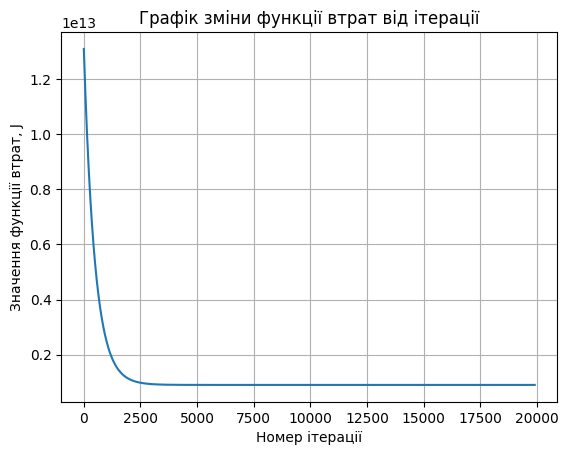
\includegraphics[width=0.6\linewidth]{hw3_files/hw3_22_0.png}
\end{center}

Аналітичний вираз для вектора вагових коефіцієнтів:

\[ \vec{w}^* = \left(\mathbf{X}^{\mathrm{T}} \mathbf{X}\right)^{-1}\mathbf{X}^{\mathrm{T}} \vec{y}. \]

Аналітичний метод надає точні значення коефіцієнтів, але для знаходження
вектора вагових коефіцієнтів за аналітичним методом потрібно обчислювати
обернену матрицю
\(\left(\mathbf{X}^{\mathrm{T}} \mathbf{X}\right)^{-1}\), що може
вимагати значних обчислювальних ресурсів. Зокрема, обчислення оберненої
матриці має складність порядку \(k^3\), де \(k\) --- розмірність матриці.
Це може бути дуже витратним з обчислювальної точки зору.

Окрім того, якщо матриця \(\mathbf{X}^{\mathrm{T}} \mathbf{X}\) є погано
обумовленою, це означає, що власні числа цієї матриці близькі до нуля.
Погано обумовлена матриця може виникнути, наприклад, коли деякі ознаки
(стовпці матриці \(\mathbf{X}\)) мають високу кореляцію або
колінеарність. У таких випадках обчислення оберненої матриці може бути
непростим завданням, і воно може стати чисельно нестійким, що призводить
до неточностей і неправильних результатів.

Отже, в реальних задачах машинного навчання, де матриця
\(\mathbf{X}^{\mathrm{T}} \mathbf{X}\) може бути погано обумовленою або
великого розміру, аналітичний метод може бути невигідним через
обчислювальну складність та чисельну нестійкість, і частіше
використовуються інші методи оптимізації, такі як ітеративні методи
(наприклад, градієнтний спуск), які є більш ефективними та стійкими до
чисельних проблем.

\begin{pythoncode}
analitical_W = np.linalg.pinv(X.T @ X) @ X.T @ Y
analitical_W
\end{pythoncode}

\begin{out}
	array([3.72448352e+02, 3.68974672e+05, 1.37031315e+06])
\end{out}


\section{Алгоритми бібліотеки \texttt{sklearn.linear\_model}}

Алгоритми реалізують метод найменших квадратів (МНК)

\begin{pythoncode}
regressor = LinearRegression().fit(X, Y)
h_sk = regressor.predict(X)
\end{pythoncode}

\subsection{Візуалізація за \texttt{sklearn.linear\_model}}

Цікаво побачити результати лінійної регресії.

\begin{pythoncode}
# Створимо маску для фільтрації даних з урахуванням фіксованих значень
f_1, f_2 = 2, 1

mask = (X[:, 1] == f_1) & (X[:, 2] == f_2)

# Обираємо відповідні значення для фіксованих ознак і передбачені значення
selected_feature = X[mask][:, 0]
h_sk_selected = h_sk[mask]
Y_selected = Y[mask]

# Гграфік залежності гіпотези від обраної ознаки за фіксованих значень інших ознак
plt.plot(selected_feature, h_sk_selected, label="Гипотеза", color='red')
plt.scatter(selected_feature, Y_selected, label="Дані")
plt.xlabel("Обрана ознака (area)")
plt.ylabel("Передбачені значення")
plt.title(f"Графік залежності гіпотези від площі (area) (за фіксованих bedrooms ={f_1} і bathrooms={f_2})")
plt.legend()
plt.grid(True)
plt.show()
\end{pythoncode}

\begin{center}
	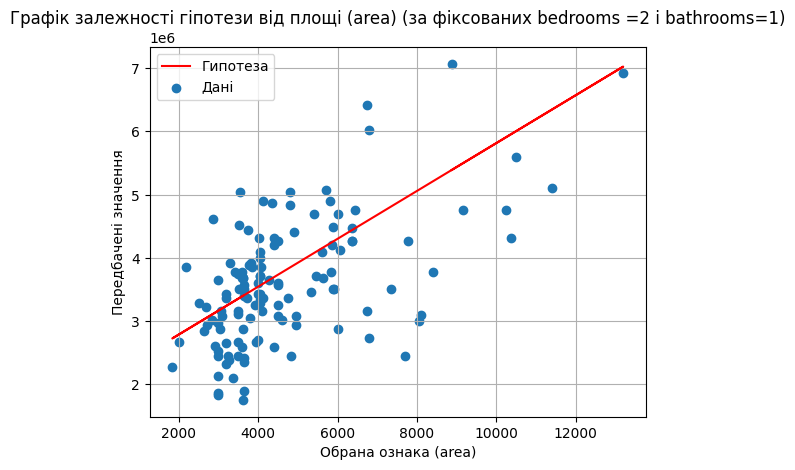
\includegraphics[width=\linewidth]{hw3_files/hw3_28_0.png}
\end{center}



\subsection{Результати}

\begin{enumerate}
	\item За ``self-made'' алгоритмом градієнтного спуску

\begin{pythoncode}
print(f"Коефіцієнти ознак (area, bedrooms, bathrooms): {coefficients}")
\end{pythoncode}

\begin{out}
Коефіцієнти ознак (area, bedrooms, bathrooms): [3.78762791e+02 4.06820872e+05
1.38604820e+06]
\end{out}

\item За аналітичним розрахунком


\begin{pythoncode}
print(f"Коефіцієнти ознак (area, bedrooms, bathrooms): {analitical_W}")
\end{pythoncode}

\begin{out}
	Коефіцієнти ознак (area, bedrooms, bathrooms): [3.72448352e+02 3.68974672e+05
	1.37031315e+06]
\end{out}

\item За МНК із бібліотеки \texttt{scisklearn.linear\_model}

\begin{pythoncode}
print(f"Коефіцієнти ознак (area, bedrooms, bathrooms): {regressor.coef_}")
\end{pythoncode}

\begin{out}
Коефіцієнти ознак (area, bedrooms, bathrooms): [3.78762754e+02 4.06820034e+05
1.38604950e+06]
\end{out}

\end{enumerate}

\subsection{Вартість квартири}

Розглянемо конкретний випадок. Зробимо передбачення ціни на квартиру яка
має характеристики \(x_1 = 7420\), \(x_2 = 3\), \(x_3 = 1\).

\begin{pythoncode}
my_X = np.array([[7420, 3, 1]])
\end{pythoncode}

\begin{enumerate}
	\item Наша функція гіпотези

\begin{pythoncode}
print(f"Ціна за квартиру {h(coefficients, my_X)[0]:.0f}")
\end{pythoncode}

\begin{out}
	Ціна за квартиру 5416931
\end{out}

\item Функція бібліотеки \texttt{scisklearn.linear\_model}

\begin{pythoncode}
print(f"Ціна за квартиру {regressor.predict(my_X)[0]:.0f}")
\end{pythoncode}

\begin{out}
	Ціна за квартиру 5243758
\end{out}
\end{enumerate}

\subsection{Висновки}

Відмінності в значеннях коефіцієнтів між методами (градієнтним спуском,
аналітичним методом і МНК) може бути зумовлена відмінностями в підходах
і параметрах кожного методу.

У цьому контексті:

\begin{enumerate}
	\def\labelenumi{\arabic{enumi}.}
	\item
	      Градієнтний спуск --- ітеративний метод, який залежить від початкової
	      ініціалізації та параметрів навчання, таких як швидкість навчання.
	      Результати можуть варіюватися залежно від цих факторів.
	\item
	      Аналітичний метод --- знаходить точне аналітичне рішення і не залежить
	      від параметрів навчання.
	\item
	      Метод найменших квадратів (МНК) --- також знаходить точне рішення і не
	      вимагає налаштування параметрів навчання.
\end{enumerate}

Відмінності у вагових коефіцієнтах можуть бути спричинені як
відмінностями в методах оптимізації, так і в особливостях даних, таких
як наявність викидів, шумів або кореляцій між ознаками. Однак важливо
зазначити, що за правильного налаштування й обробки даних відмінності в
коефіцієнтах між цими методами мають бути незначними, і всі три методи
мають давати схожі результати в контексті лінійної регресії.




% Add a bibliography block to the postdoc



\end{document}
